\section{Confidential Computing (CC)}
\label{ch:confidential-computing}

Data can be in three distinct states: ``at rest'', ``in transit'', and ``in
use''. These three states describe data that lies in persistent storage,
traversing the network, and data that is currently being processed. While
technologies in order to protect data ``at rest'' and ``in transit'' are
commonly used today, there are not many methods to protect data ``in use''.

By executing computations in hardware-based trusted execution environments (see
section \ref{sec:TEE}) confidential computing (CC) protects data ``in use''. In
order to assure a client that the requested environment can be trusted, remote
attestation protocols (see section \ref{ch:remote-attestation}) are used. The
combination of these two practices enable service providers to offer trusted
services that can be verified remotely by clients or third-parties.

\subsection{Trusted Execution Environments (TEEs)}
\label{sec:TEE}

\subsubsection{Properties}

There are different definitions of a trusted execution environment (TEE) with
varying properties. We will focus on the properties needed to build a platform
where securing client data and building trust is the main concern. These
properties are:

\begin{description}
  \item[Data confidentiality]
    Prevent unauthorized entities to view data that is in use within a TEE
  \item[Data integrity]
    Prevent unauthorized entities to add, remove, or change data while it is in
    use within a TEE
  \item[Code integrity]
    Prevent unauthorized entities to add, remove, or change code executing in the
    TEE
\end{description}

\todo[inline]{Explain why these three properties are important in order to build trust}

\subsubsection{Why hardware-based TEE}

The security of a software layer can only be as strong as the layers below it.
This is why an ideal security solution acts from the lowest layer possible. By
providing security through the lowest layer -- the hardware -- it is possible to
remove almost all layers below the TEE from its TCB. This includes the
infrastructure provider, host operating system, hypervisor, service provider,
and platform the TEE is running on. The only component remaining in the TCB of
the application is the hardware providing the TEE properties.

Utilizing software-based TEEs would mean giving control of enforcing TEE
properties in the hands of the service provider, conflicting with goal
\subGoalRef{2}{1}. For this reason this paper will focus solely on
hardware-based TEE technologies.

\subsection{TEE Models}

There are two distinct models of TEEs, process-based and VM-based.

\subsubsection{Process-based TEEs}

Process-based TEEs introduce a new programming model. A program needs to be
split into two components, trusted and untrusted. These are often referred to as
the ``enclave'' and ``host''. The enclave is executed in an environment where
all TEE properties are provided. The enclave component should contain all code
that interacts with sensitive data, whereas the host component is responsible
for handling non-sensitive tasks like networking and file I/O.

While the host is not shielded the enclave is protected from the rest of the
system, this includes

\begin{itemize}
  \item the enclave's own host
  \item other processes
  \item the operating system
  \item the bootloader and firmware such as the BIOS
  \item the hypervisor and host operating system (in virtualized environments)
  \item hardware other than the processor
\end{itemize}

\todo[inline]{Go into detail about how process-based TEEs work?}

Splitting a program into enclave and host is challenging. It requires a deep
understanding of security and how these process-based TEE solutions work. To
ease the development of such applications SDKs and frameworks often hide the
split between host and enclave from the developer\cite{schuster2022}.

Library OSes like Gramine and Occlum go even further and provide a POSIX-like
runtime environment with support for network, file I/O, and multithreading.
These library OSes contain the whole application in the enclave. But because the
enclave doesn't have access to the OS running the program, the library OS
provides libraries which implements OS system calls as library functions. This
library then interfaces with a boilerplate host for I/O\cite{tsai2014}.

Even though these SKDs, frameworks, and library OSes ease the development and
make porting of existing applications easier, using process-based TEEs still
requires more development effort and modifications of existing applications.

\todo[inline]{Example: Intel SGX}

\subsubsection{VM-based TEEs}

The main concept of VM-based TEEs is to apply the TEE properties to a full
virtual machine running on top of a VMM. This enables VM-based TEEs to run
basically any application without modifications. While VM-based TEEs have a
larger TCB than process-based TEEs they are still explicitly designed to protect
workloads from underlying software layers.

\todo[inline]{Example: AMD SEV}
\todo[inline]{Example: Intel TDX}

\subsubsection{Comparison}

Figure \ref{figure:cc-tee-comparison} shows a simplified comparison between the
TCBs of an application running without CC, inside a process-based TEE, and
inside a VM-based TEE.

\begin{figure}
  \centering
  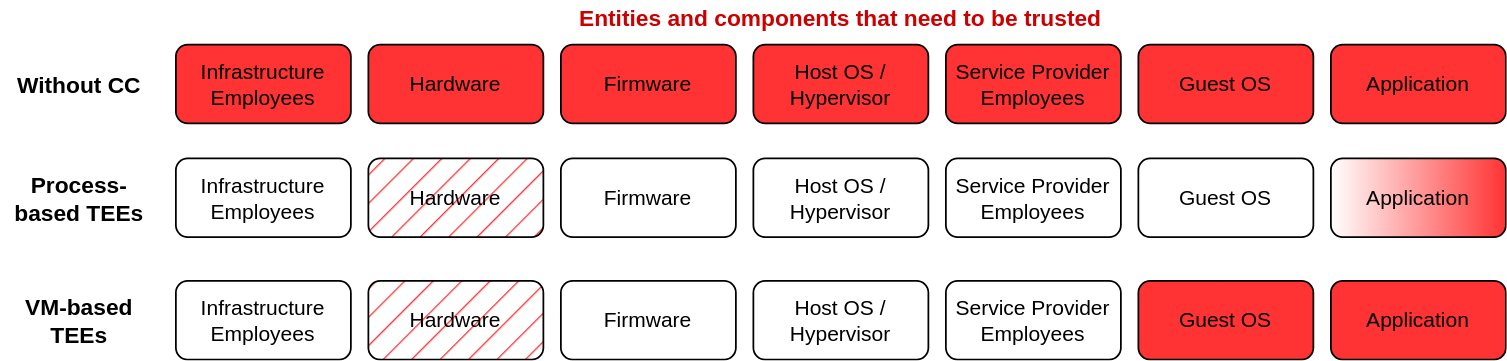
\includegraphics[width=\linewidth]{resources/cc-tee-comparison.png}
  \caption[Comparison of trusted execution environment models]{
    Comparison of TEE models. Boxes marked in red highlight entities and
    components that have to be trusted. In both TEE models the CPU still
    enforces the TEE properties and thus still has to be trusted. In the
    process-based TEE the application is marked with a gradient because the
    application has to be split into two parts.
  }
  \label{figure:cc-tee-comparison}
\end{figure}

\subsection{Problems}

\subsubsection{Support for accelerators}

\todo[inline]{Reference the heavy use of accelerators in ML}
\todo[inline]{Explain ongoing effort without going too much into detail (Reference CRONUS)}
